% !TEX root = ./../main.tex
\chapter{MD tools, parallelization and hardware acceleration}
%Manuale GROMACS 3.17.5 PP/PME ranks
%http://www.gromacs.org
Different tools for setting up an \ac{MD} simulation, a metadynamics run and to analyze the collected data exist. In this Chapter we present the main tools used in this thesis: the \href{http://www.gromacs.org}{\gromacs} and the \href{http://www.plumed.org}{\plumed} packages. Moreover, with the increasing of the systems complexity, different \textit{parallelization} techniques are developed in order to exploit all the computational resources of the modern multi--core CPUs and multi--node cluster. We shall describe the main used in this thesis work. Then we give the main input parameters used to setup the \ac{MD} and metadynamics runs. 


\section{GROMACS package}
The \ac{MD} tool and the main analysis tool used in this thesis work is the \href{http://www.gromacs.org}{\gromacs} \cite{gromacsManual} package. It is compatible with both atomistic and \ac{CG} \acp{FF} and support a variety of options and parameters such as different thermostat and barostat algorithms, different methods to treat the electrostatic interaction such as the \ac{ESM} and the \ac{PME} method, different integrators, cut--off schemes and so on. For what concern the trajectory analysis it holds a comprehensive framework for obtaining different quantities. Moreover it supports different kind of parallelization techniques that is, it has the compatibility with both multi--core single processor (home PC) and multi--core multi--processor (cluster) architectures with the support of both \href{https://computing.llnl.gov/tutorials/mpi/}{MPI}
%\footnote{https://computing.llnl.gov/tutorials/mpi/} 
and \href{https://computing.llnl.gov/tutorials/openMP/}{OpenMP}
%\footnote{https://computing.llnl.gov/tutorials/openMP/}
libraries for the inter--nodes and inter--cores information exchange and the support of different hardware accelerated frameworks such as \href{https://developer.nvidia.com/cuda-zone}{NVIDIA CUDA}\textsuperscript{®}
%\footnote{https://developer.nvidia.com/cuda-zone}
, \href{https://www.khronos.org/opencl/}{OpenCL}™
%\footnote{https://www.khronos.org/opencl/}
 and \href{http://www.openacc.org}{OpenACC}.
 %\footnote{http://www.openacc.org}  

\subsection{Parallelization}
Parallelization refers to the possibility of running a program, in this case an \ac{MD} simulation, in parallel with the use of more then one CPUs or more then one cores per CPU or both. The efficiency of a parallelization scheme is mainly determined by how much information each core and/or CPU has to exchange with the others, the least the better. The reason is that the libraries (MPI and OpenMP) needed for the exchange of the information are not fast as the cores are. Hence when the waiting time for the information exchange becomes higher than the total time spent in executing the parallel code, the program has reached its scaling limit, that is, no more cores have to be used.

For what concern an \ac{MD} simulation there exists one main kind of parallelization scheme: the domain decomposition. It exploits the local character of most of the interactions used in common \acp{FF}. The simulation box is dived into cells, each of which is assigned to a cores such that it store only a portion of the whole system: the particles which lie in that region and forces between them and the atom positions and forces from neighboring regions owned by other cores. In order to minimize the communication between different cores each cells has to minimize its surface respect to the volume, so it is important to use cells that are as cubic as possible. Indeed if the cells are not too small, the particle update can be carried out every time the neighbor list is updated and not avery \ac{MD} step. Then, this also contribute to reduce the number of communications. A common choice is to use cell greater than two times the cut-off radius. The scaling limit with the domain decomposition is reached when the cells are so small that a few number of particles lied in each cell; for \gromacs it means $\sim 100 \div 200$~atoms/core.

\subsection{PP and PME nodes}
When using the \ac{PME} method for the electrostatic interaction a special parallelization scheme is needed in order to speed up the simulation. The reason is related to the fact that the \ac{PME} method intrinsically need to know all the particle positions in the whole simulation box. In a domain decomposition scheme this results in a massive use of the so called \textit{all--to--all} communications, i.e. all cores have to communicate to each other. Hence this leads to a loss of computational performance. In order to minimize the all--to--all communications, \gromacs implement the possibility to assign a subset of the cores exclusively to the calculation of the energy contribution of the electrostatic interaction using the \ac{PME} method, while the rest of the work is assigned to the remaining cores, called the \ac{PP} cores. 
\begin{figure}[h!t]
	\centering
	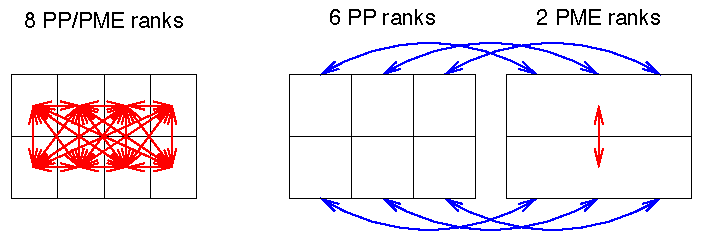
\includegraphics[width=0.8\textwidth]{./img/PMENodes}
	\caption{Left: example of the use of $8$ cores for both \acs{PP} and \acs{PME}. Right: same but $2$ cores are used only for \acs{PME} and the other for the \acs{PP} contribution. Red arrows represent the all--to--all communications while the blu arrows are the communications between one \acs{PP} core and one \acs{PME} core. Taken from \cite{gromacsManual}.}
	\label{fig:PMENodes}
\end{figure} 
In figure~(\ref{fig:PMENodes}) a schematic view of the all--to--all communications needed in a comparison between \ac{PP}/\ac{PME} in the same cores and the use of the separate \ac{PME} cores is shown. As one can see the all--to--all communications (red arrows) are smaller for the separate \acs{PME} scheme then that for \ac{PP}/\ac{PME} scheme. With this parallelization scheme the workflow of figure~(\ref{fig:PPCore}) is updated to one shown in figure~(\ref{fig:PPPMECores}). 
\begin{figure}[h!t]
	\centering
	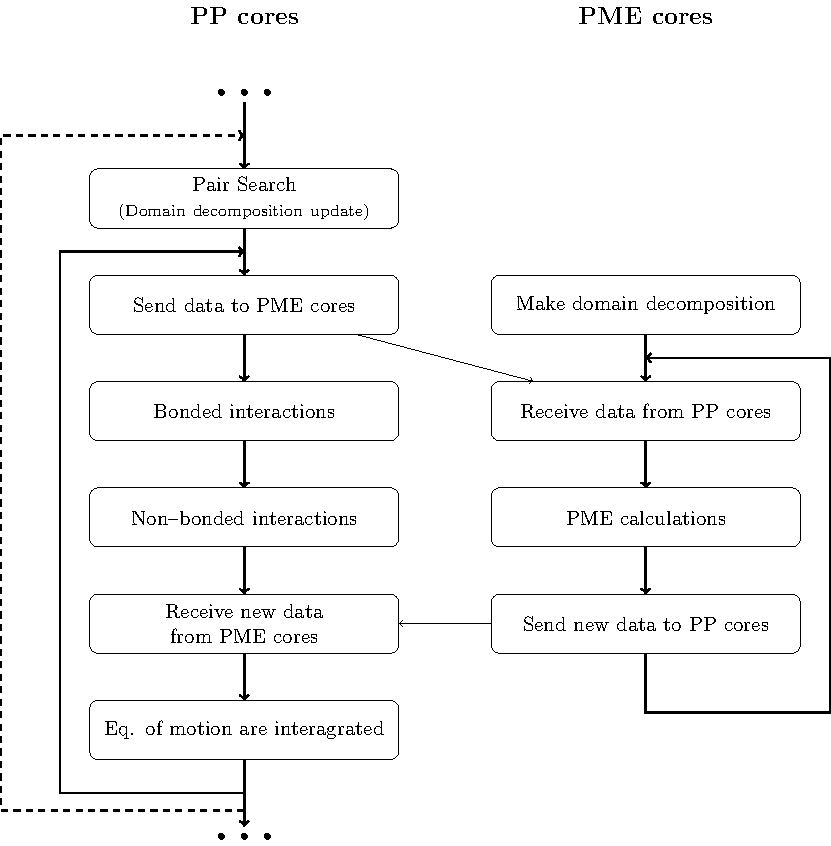
\includegraphics[width=0.8\textwidth]{./img/Schemi/PPPMECores}
	\caption{Schematic workflow of the load balancing between \acs{PP} and \acs{PME} cores.}
	\label{fig:PPPMECores}
\end{figure}

\paragraph{\textbf{PME Domain decomposition}} To optimize the load in the \ac{PME} cores a domain decomposition is still used but with a $2$D or a ``pencil'' scheme. This because the \ac{FFT} method is very inefficient if parallelized with too many cores due to the all--to--all communications, thus the domain decomposition acts on the $xy$--plane while the $z$ axis is assigned to one core; pencil refers to the shape of the domain at high parallelization. Moreover the number of domains along the $x$ axis have to be equal to the number of domains in the \ac{PP} decomposition and eventually a $1$D scheme can be used along the $y$ axis only if the \ac{PP} decomposition has one domain along $x$ axis. To avoid superfluous communication of coordinates and forces between the \ac{PP} and \ac{PME} cores, the number of cells along the $x$ axis should ideally be the same or a multiple of the number of the \ac{PME} cores. Most of this issues are taken into account approximately automatically by \gromacs at the begging of the simulation.

\paragraph{\textbf{PP -- PME load balancing}} In order to achieve the better performance a well balancing of the load between \ac{PP} and \ac{PME} cores is needed, i.e. no core should expect to each other. In \gromacs this is done balancing the real part and the \ac{PME} part of the electrostatic interaction. Since the real part is computed on \ac{PP} cores as non--bonded interaction, changing the Coulomb cut--off between the real and the \ac{PME} part, will adjust the load balancing between \ac{PP} and \ac{PME} cores. Off course this has to be done keeping unchanged the desired accuracy of the electrostatic energy contribution. In \gromacs the ratio between the starting cut-off radius and the \ac{PME} grid spacing gives the accuracy of the electrostatic energy contribution. Then changing both the Coulomb cut--off and \ac{PME} grid spacing, leaving the ratio unchanged, will adjust the \ac{PP} -- \ac{PME} load without affecting the accuracy. We have to stress out that at the begging of the simulation the Coulomb, the Van der Waals and the pair list cut--off radii must be the same. Then \gromacs only adjust the ratio between the Coulomb cut--off and the \ac{PME} grid spacing, without affecting the cut--off of the pair list or of the Van der Waals interaction.

\subsection{Hardware acceleration}
Excluding the \ac{PME}, an other most time consuming part of an \ac{MD} simulation, is the computation of the non--bonded interactions. The way to speed up the simulation without recur to more cores, because, for example, the system has reached its scaling limit or there are no longer cores, is to use an hardware accelerator. By offloading the computation of the non--bonded interactions to the hardware accelerator, the CPU has the possibility to do \textit{in concurrency} other calculations such as the \ac{PME} calculations. \gromacs support completely the NVIDIA GPU with the NVIDIA CUDA\textsuperscript{®} framework acceleration together with the use of the Verlet cut--off scheme. Other GPUs or other cut-off scheme are partially supported with OpenCL or OpenACC libraries. 

The speed up of the simulation by offloading the non--bonded interactions to a GPU using NVIDIA CUDA\textsuperscript{®} is of the order of two or three times faster than that of a non accelerated simulation. Moreover, to increase the performance, avoiding the waiting time of the CPU for the GPU to finish the non--bonded calculations, the same load balancing between \ac{PP} and \ac{PME} part can be used. Adjusting both the Coulomb cut--off and \ac{PME} grid spacing, leaving the ratio unchanged, will adjust the load between the real and the reciprocal part of the electrostatic energy contribution. Since the real part is computed in the GPU as non--bonded interaction, it will adjust the load balancing between the GPU and the CPU. Using an hardware accelerator the schematic workflow of figure~(\ref{fig:PPCore}) is updated to one shown in figure~(\ref{fig:GPU}).

Basically and briefly the main difference, as showed in figure~(\ref{fig:GPUvsCPU}), between a CPU and a GPU is the total number of 
\begin{figure}[h!t]
	\centering
	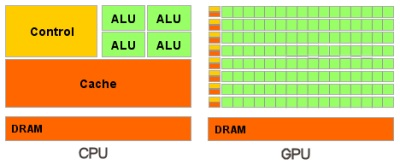
\includegraphics[width=0.6\textwidth]{./img/GPUvsCPU}
	\caption{Schematic comparison between a CPU and a GPU.}
	\label{fig:GPUvsCPU}
\end{figure}
\textit{computing modules} assigned to do vectorized calculations i.e. calculation that involve many vectors of different length. Now days the total number of hardware cores in a high level CPU is eight cores. Instead, a middle level GPU has a number of computing modules of the order of $ > 10^3$. In the GPU case, the computing module is essentially a \ac{SIMD} computing unit which is composed by several cores which each of it is equipped by several \acp{ALU} and \acp{FPU}. A \ac{SIMD} unit is a specific module for vector calculation: it give several instruction set to perform the same instruction on a multiple data stream i.e. multiple data arranged in a vector fashion. In figure~(\ref{fig:simd}) a schematic representation of a \ac{SIMD} that execute in parallel four two number sums
\begin{figure}[h!t]
	\centering
	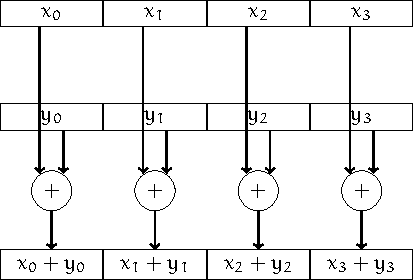
\includegraphics[width=0.5\textwidth]{./img//simd/simd.pdf}
	\caption{Block diagram of a \acs{SIMD} computation on a four element vectors.}
	\label{fig:simd}
\end{figure}
i.e. the sum of each cell of the two vectors, is shown. Essentially this is possible thinking a $32$--bit register as vector of four $8$--bit or two $16$--bit numbers, then the same instruction is applied to each cell pair of the vectors. Even a modern CPU has the possibility of \ac{SIMD} computation but the goal of the GPU implementation is the extremely high number of modules arranged in a efficiency pipeline, respect to CPU one. Hence the \textit{concurrency} calculations on a streamed data are much faster if executed on a GPU then on a CPU. On the contrary the CPU has the ability to perform several task in parallel (or approximately in parallel).
\begin{figure}[h!t]
	\centering
	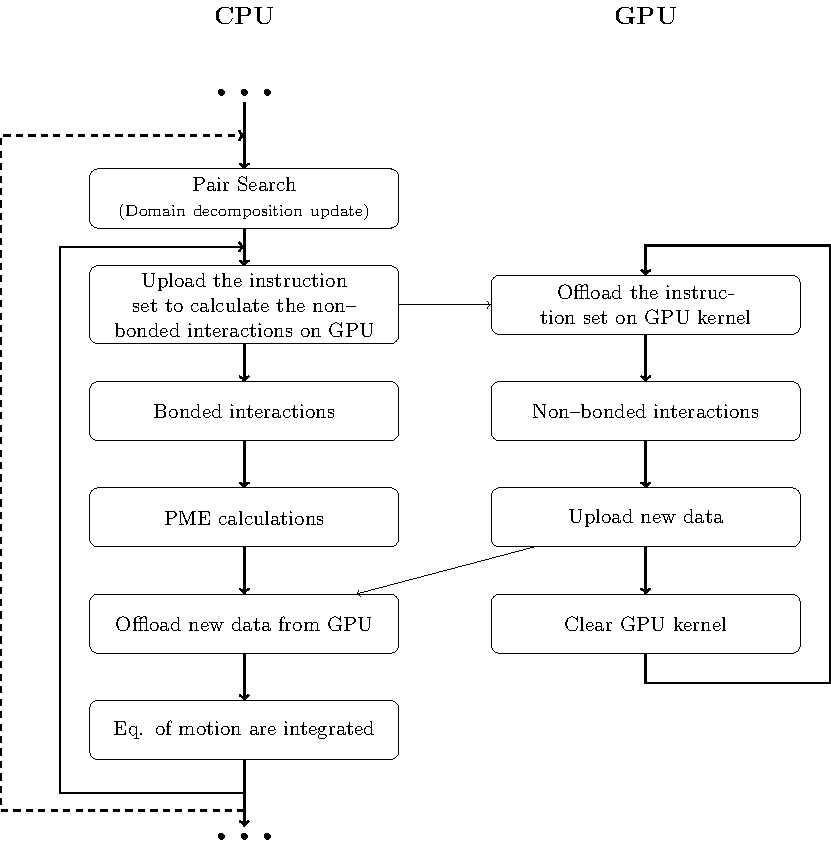
\includegraphics[width=0.8\textwidth]{./img/Schemi/GPU}
	\caption{Schematic workflow of the calculation of the interactions with the use of a GPU as hardware accelerator.}
	\label{fig:GPU}
\end{figure}


\section{PLUMED package}
The tool used for setting up and analyze a metadynamics simulation is the \href{http://www.plumed.org}{\plumed} package. It is an open source project composed by a set of libraries used for analyze the data obtained with a metadynamics simulation (first all, for obtaining the \ac{FES} from the history--dependent bias potential) or other advanced sampling technique, such as umbrella sampling. Moreover it works together with the most popular \ac{MD} tools, \gromacs included. In that sense it is a sort of plug--in that insert the advanced sampling code and algorithms inside the main \ac{MD} loop of the used \ac{MD} tool.

For setting up a metadynamics simulation \plumed require an input file in which we have to specify what are the \acp{CV} and the parameters to be used in the metadynamics run. Moreover there is the possibility to add more feature such as, online analysis or more output files and options.

For what concern the parallelization we have noted that it is badly parallelized between more than one node, that is, we observe good computational performance if we use the parallelization between cores inside the same CPU with the OpenMP library and the use of the GPU as hardware accelerator. Otherwise, for example with more than one node of a cluster, we obtain worse computational performance. Moreover, depending on the system and the parameters of the metadynamics, we observe a general decrease of computational performance compared to an un--biased \ac{MD} simulation.

Below we show a typical input file used in this thesis work for a metadynamics simulation.
\begin{Verbatim}[fontsize=\scriptsize,xleftmargin=1cm]
# global variable: z distance from COM of particles 385-7040 and paticle 308 
memb: COM ATOMS=385-7040
mus: COM ATOMS=308
dist: DISTANCE ATOMS=memb,mus COMPONENTS

# Activate metadynamics in dist.z
METAD ...
LABEL=metad
ARG=dist.z 
PACE=50000
HEIGHT=2.479
SIGMA=0.06
FILE=HILLS
GRID_MIN=-9
GRID_MAX=9
GRID_SPACING=0.005
... METAD

# monitor the two variables and the metadynamics bias potential
PRINT STRIDE=10000 ARG=dist.z,metad.bias FILE=COLVAR
\end{Verbatim}

\section{Simulation parameters}
Since \gromacs is compatible both with atomistic and \ac{CG} \acp{FF} and with different kind of \ac{MD} simulations, such as with a $NVE$ or $NVT$ or $NpT$ ensemble, different \ac{MD} integrators, different algorithms to treat the long-- and short--range interactions and so forth, few input files must be given at \gromacs input. Briefly these input files are the initial configuration file in which the position and eventually the velocity of all particles and the three box dimensions are saved; the input parameters file in which, following the \ac{FF} receipt, all the \ac{MD} parameters are given; the topology file in which all the particles of a system are described: what kind of forces between them, the assigned charge, the mass and all the constant refer to the particles and the interactions between them, even this file, generally, is created under the receipt of the \ac{FF} used.

In table~(\ref{tab:inputParam}) we report the most important \ac{MD} parameters used in this thesis work. In table~(\ref{tab:inputParam}) ``VbT'' means Verlet--buffer--tolerance; ``VdW'' means Van der Waals; $T$ and $p$ coupling are the thermostat and barostat algorithms used, respectively; $\tau_T$ and $\tau_p$ are the related time constants; $p$ type, is the pressure coupling type: semi--isotropic means two independent pressure coupling for $xy$ axes and for $z$ axis; $K$ is the related compressibility (in this case equal for both pressure coupling). In general when starting an \ac{MD} simulation, an equilibration run (Eq. in table~(\ref{tab:inputParam})) of few nanoseconds, that also generate the random velocities from the Maxwell–Boltzmann distribution at fixed temperature, is needed for equilibrating the volume of the simulation box and the whole system. Then one have to switch to the production run (Run in table~(\ref{tab:inputParam})) in which the correct ensemble is sampled. 

For what concern the metadynamics parameters, in accordance with \cite{ourPaper}, in table~(\ref{tab:metadynParam}) we report the main input parameters used to set up a metadynamics run.

\begin{table}[h!t]
	\centering\footnotesize
	\begin{tabular}{lcccc}
		\toprule
		Input parameter & Eq. \acs{PME} & Run \acs{PME} & Eq. \acs{PME}\&\acs{PW} & Run \acs{PME}\&\acs{PW} \\ \toprule
		Time step [fs]		& $10$ & $20$ & $5$ & $20$ \\ \midrule
		cut--off scheme		& Verlet & Verlet & Verlet & Verlet \\ \midrule
		VbT [J/(mol ps)]	& $5$ & $5$ & $5$ & $5$ \\ \midrule
		Coulomb Type		& \acs{PME}	& \acs{PME}	& \acs{PME} & \acs{PME} \\ \midrule
		$r$ Coulomb	[nm]	& $1.2$ & $1.2$ & $1.2$ & $1.2$ \\ \midrule
		$\varepsilon_r$		& $15$ & $15$ & $2.5$ & $2.5$ \\ \midrule
		\acs{PME} grid [nm]	& $0.12$ & $0.12$ & $0.12$ & $0.12$ \\ \midrule
	    \acs{PME} order		& $4$ & $4$ & $4$ & $4$ \\ \midrule
		VdW type			& cut--off & cut--off & cut--off & cut--off \\ \midrule
		$r$ VdW [nm]		& $1.2$ & $1.2$ & $1.2$ & $1.2$ \\ \midrule
		$T$ coupling		& $v$--rescale & $v$--rescale & $v$--rescale & $v$--rescale \\ \midrule
		$T$ [K]				& $310$ & $310$ & $310$ & $310$  \\ \midrule
		$\tau_T$ [ps]		& $2.0$ & $2.0$ & $2.0$ & $2.0$ \\ \midrule
		$p$ coupling		& Berendsen & Parrinello--Rahman & Berendsen & Parrinello--Rahman \\ \midrule
		$p$ type			& semiisotropic & semiisotropic & semiisotropic & semiisotropic \\ \midrule
		$p$ [bar]			& $1.0$ & $1.0$ & $1.0$ & $1.0$ \\ \midrule
		$\tau_p$ [ps]		& $4.0$ & $12.0$ & $4.0$ & $12.0$ \\ \midrule
		$K$ [bar$^{-1}$]	& $4.5\cdot 10^{-5}$ & $3.0\cdot 10^{-4}$ & $4.5\cdot 10^{-5}$ & $3.0\cdot 10^{-4}$ \\ \midrule
		$v$ random			& yes ($310$~K) & no & yes ($310$~K) & no \\ \bottomrule 
	\end{tabular}
	\caption{Summary of the main input parameters used in my \acs{MD} runs.}
	\label{tab:inputParam}
\end{table}

\begin{table}[ht]
	\centering
	\begin{tabular}{llll}
		\toprule
		Deposition pace ($\tau$) & Gaussian height ($w$)& Gaussian width ($\delta s$) & Grid spacing \\ \toprule
		$50000$ \ac{MD} steps$^a$ & $2.479$~kJ$^b$ & $0.06$~nm & $0.005$~nm \\ \bottomrule
	\end{tabular}
	\caption{Main metadynamics parameters used in this thesis work. \footnotesize $^a$ With a $20$~fs time step it means a deposition of a Gaussian every nanoseconds. $^b$ At thermostat's temperature it is approximately equal to $1~k_BT$.}
	\label{tab:metadynParam}
\end{table}


